
\section{Motivation}
% general motivation
With the ever-growing amount of data on the Internet, it has become increasingly difficult to deal with information overload. A recommender system finds patterns in data and tries to analyze the behavior and preferences of users to recommend information that appears most relevant to a particular user and filter out unrelated noise~\cite{isinkaye2015recommendation}. Over the years, recommender systems have evolved to accommodate a wide range of problems.

% why recommender systems - specifically as an example in e-commerce
\paragraph{Need to Filter Choices: Recommendations}
In the context of e-commerce, advertising plays a crucial role. When consumers face too many choices, they experience anxiety~\cite{schwartz2004doing}. Recommender systems target consumers with advertising to reduce the available options and recommend products. By making effective recommendations, the advertiser can increase the number of sales.
Products otherwise found only by extensive searches are made readily available to the consumer~\cite{rohde2018recogym}. Recommender systems are present in all areas of the Internet. When one performs a Google search, Google's PageRank algorithm recommends the best matching websites to our search query. Behind the scenes, search engine optimization (SEO) is a research area focused on increasing the ranking for specific websites to appear higher in the search results, which in turn generates more traffic. And most social media platforms feature a dedicated page for users to explore recommended and related content, which can be in the form of videos, images, or users to follow.

\paragraph{Too much Noise and too few Patterns}
The massive amount of data that is out there contains a large number of patterns that a system can extract. Yet, one of the main challenges nowadays is not so much to capture patterns in large amounts of data: the difficulty lies in capturing patterns in small portions of data. Taking the example of a social media network such as Reddit, the system should then already make recommendations to a new user who has only visited one post.

% need to decide what to look at
Modern architectures are undoubtedly challenging: on the one hand, the information passed can be minimal, and on the other hand, the information to learn from is often of vast proportions. Hence, the recommendation problem at its core is a problem of attention. Based on the available information, the system needs to decide where to put the focus. The system also needs to determine, how many resources to allocate to inspect the subspace.


\section{Requirements}

% distracted by mass
Although information in general is abundant, \emph{relevant} information is often scarce and very much obscured by the irrelevant mass. Faced with this scarcity, it appears natural when trying to optimize recommendations to try to augment the information available by all means. Taking into account sequences of data points instead of just isolated items, in the form of sequential embeddings~\cite{Githubbert4rec, tang2018personalized, rendlefactorizing} has been a recent important step in that direction, out of many.

\paragraph{Need to include Temporal Patterns}
%
Fortunately, there are still plenty more patterns in the data one can draw more information from. The temporal order of data holds valuable information. When patterns change, the system ought to adapt. It should keep up with current patterns and predict upcoming patterns in the near and further future to allow for effective optimization ahead of time. For example, a user's behavior evolves continually due to changes in mood (short term) or changes of taste (long term). The system should identify and process the change and adapt to it: forget old patterns and effectively learn new patterns~\cite{tsymbal2004problem}. The same can happen for a larger group of users with data that exhibits spatio-temporal patterns.

Existing work in recommendations only captures the sequential patterns in a time-agnostic fashion: $ A $, $ B $, $ C $ instead of $ A(t=0s $), $ B(t=10s) $, $ C(t=50s) $, for example. A mechanism to bring together timestamp values and sequential patterns thus appear necessary~\cite{wang2019survey, wang2019sequential}.

\paragraph{Need for Integration in a Heterogeneous Environment}
%
Another important aspect is that data is not isolated but is part of a highly heterogeneous ecosystem: users query the system, administrators want to change and control the systems. Then there is new data constantly added to the system. The ecosystem that makes up the data is highly unstructured. Such a large variety of events calls for a differentiated and flexible mechanism to model sequential patterns in a hybrid environment.  Rather than a simple interface with user sequences fed in without consideration for the types of the events, as is predominant in the literature~\cite{sun2019bert4rec}, we need a solution that can smoothly integrate the different forms of events.

There is a need to extend the mechanism that captures the sequences to broaden the spectrum of observations. Multiple forms of capture need to be combined. For example, the queries from users need to encode particularities. Queries from analysts should be encoded differently, given that they have other semantics. 


\paragraph{Need for Explainability through Flexibility}
%
A considerable challenge is to build a system that is both reliable and explainable to users. Only then can humans be brought on board, and their valuable input fit into the model. Collaboration between humans and machines is necessary for the system to capture the semantics of the data in depth---only then can AI's full potential come to fruition.

Existing work is by and far agnostic to the massive diversity of relationships between objects. The state of the art does not capture the relationship among different categories of data~\cite{sun2019bert4rec}. But, further, the relations are often opaque black boxes without any control mechanism. A hybrid approach that offers controls and makes use of various mechanisms is needed.

Existing work is by and far agnostic to the massive diversity of the relationship between objects. The state of the art does not capture the relationships among different categories of data~\cite{sun2019bert4rec}. Not only are diverse relationships poorly captured in a differentiated manner but they are also not presented to humans in an understandable manner: the mechanisms are opaque black boxes without any clear lever. A hybrid approach that offers controls rooted in the diversity of the environment is needed.
% A hybrid approach that offers controls rooted in the diversity of the environment is needed.
% to be defined what means

To get the full expressivity of data and integrating its diversity organically, capturing relevant substructures is paramount and there, given the combinatorial number of entities involved, effective summarization becomes a necessity: mechanisms are needed to continuously decide which substructures should receive which representation and how many resources to allocate. Over time one should review the decisions: merging, shrinking and extending substructures as necessary. Existing work is still far from such organic, highly adaptive, and highly dynamic structures, as the data is typically only represented with flat (vs. hierarchical and organic), undifferentiated~\cite{sun2019bert4rec} (vs. summarized) structures.

% effective summarization = final embedding from classic, off general classic embeddings
% general classic embeddings possibly completed by ML embeddings


\section{Problem statement}
State-of-the-art models lack a comprehensive, time-aware solution (sequential and by value) that flexibly captures data patterns. There is a need for a tractable plurality of forms of capture and associated controls and the data representation ought to be organic and capture the relevant patterns.
%
Considering these gaps, we offer to address the following problem in this work:

\emph{
How to capture data in a fully temporally aware manner and with organic controls?}


\section{Solution}
%
We propose a comprehensive solution that captures the temporal evolution of sequential dependencies in the data. A novel hybridization mechanism combines several state-of-the-art machine learning models as well as a novel solution with organic control by organizing the models in a graph of sketches.
%
Via an automated learning mechanism, the system learns to adapt parameters to changing patterns in the data, within a frame defined by a human---hence balancing resources spent in human control vs. in machine exploration.
% integrating user control to maximize flexibility and organically summarize data at runtime, classically with guarantees and with learned models, in a balanced mix.
% TODO. discuss the optimization of the parameters in frame def. by humans
% not in current design


%% Figure left for later
% We present our design in Figure~\ref{fig:system_design_hybridization}.

% \begin{figure}[htbp!]
%     \includegraphics[width=.5\columnwidth]{images/handdrawn_system_design_universal_Bert_p1.jpg} % = more the online aspect. Will all be on one diagram anyway.
%     \includegraphics[width=.5\columnwidth]{images/handdrawn_system_design_universal_Bert_p2.jpg} % = more the online aspect. Will all be on one diagram anyway.
%     \caption{Sketch of our hybrid system design.}
%     \label{fig:system_design_hybridization}
%     % got to agree on sth. here
% \end{figure}
%
% 

\subsection{Online Inference---Integration of Temporal Evolution}
Our workload consists of a sequence of queries from a variety of users. Queries are parsed%
% (streaming) %
and batched. Our system then issues recommendation on the batch%
% (online)
% . Another batch, possibly larger, is passed to train on.

% We illustrate our online processing in Fig.~\ref{fig:system_design_hybridization}
% by how the embedding updates from each batch (bottom) propagate through propagate through our pipeline (upwards). % reference assumes diagram dawn

%
% The learned word embeddings determine the summarization, which is our basis for starting with the next window.


% re-use
%    graphs/hybrid_GCN_full_info_flow
%    https://docs.google.com/drawings/d/1bG0AhnmaR18W5fCU77Xq-joFDVWkBeDfwvCnuldDLmo/edit?usp=sharing but with sequences per user?
%   (@Su's)
% %
% I think combined with
%    sets/classic_full_system_workflow
%    https://docs.google.com/drawings/d/1SBWWLdSUzSB5RltQSCVpC-GtDUUEuRhqwEwmDBLLwlY/edit?usp=sharing
%   (@Nebi's)
% , combining extrinsic and intrinsic into one graph
% for the user-driven sequence aspect
% possibly overkill
% % 
% TODO Nebi: deliver a more detailed and more process-close diagram like
%    sets/Classic_Intrinsic_Summarization_TF-IDF_Vectorizer
%    https://docs.google.com/drawings/d/1Re5U5lHkBNrNGkZ_TBBG_8KIBv85o6QEnzy1uki3UEI/edit?usp=sharing
%   (@Nebi's)
% but for extrinsic and not for intrinsic. Will be drawn the coming days anyway, since Nebi gotta hand in these days.
% -> then we can reuse that sets/classic/extrinsic diagram here in sets/ML. In particular we split per user in sets/classic/extrinsic and that'd fitvery well 
% 
% 

\subsection{Integration of Control to Trade-off Classic/ML}
The system combines classic Markov-chain-driven approaches and ML-driven inference solution as a basis to build embeddings from, with a combination logic on top.
% ---Figure~\ref{fig:classic_conceptual_diagram}---.
Our hyperparameter optimization logic optimizes the parameters but within the frame set by the user, hence trading off control from user vs. resources spent on learning. To save space, ensure an understandable control and improve our performance, the items are summarized into substructures.
%
% now rather thinking we will mimic classic structurally in the hierarchy of sketches involved, i.e., take over the organic summarization and control of resources from classic.
% Simultaneously, we will reuse the embedding computation from classic as a basis to build our embeddings from, just as one solution among others.
% 

% % would be fine with us dropping the diagrams altogether to save time
% % can be in the final thesis anyway.
% % But one way or another, our diagrams will be mixes of those, just because our pipelines inherit so much from these. 
% % 

% \begin{figure}[ht]
%     % diagram showing classic (extrinsic + intrinsic)
%     % should be small and not sold too much since we use it here but don't 
%     % develop it
%     \includegraphics[scale=.5]{images/diagrams/classic_conceptual_diagram}
%     \caption{Sketch of our classic design (internal work).}
%     \label{fig:classic_conceptual_diagram}
%     % take from
%     %    sets/classic_full_system_workflow
%     %    https://docs.google.com/drawings/d/1SBWWLdSUzSB5RltQSCVpC-GtDUUEuRhqwEwmDBLLwlY/edit?usp=sharing, combining extrinsic and intrinsic into one graph
%     % for the user-driven sequence aspect
% \end{figure}


% \begin{figure}[ht]
%     % diagram showing classic (extrinsic + intrinsic)
%     % should be small and not sold too much since we use it here but don't 
%     % develop it
%     \includegraphics[scale=.5]{images/diagrams/classic_conceptual_diagram}
%     \caption{Sketch of our classic design (internal work).}
%     \label{fig:classic_conceptual_diagram}
%     % take from
%     %    graphs/hybrid_GCN_full_info_flow
%     %    https://docs.google.com/drawings/d/1bG0AhnmaR18W5fCU77Xq-joFDVWkBeDfwvCnuldDLmo/edit?usp=sharing but with sequences per user?
%     %   (@Su's)
%     % for the embedding hybridization aspect
% \end{figure}



% no
% \begin{figure}[!ht]
%     \includegraphics[width=1.0\columnwidth]{images/BERT4Rec_workflow.png}
%     \caption{BERT4Rec combined with textual content embeddings}
%     \label{fig:system_design_universal_Bert}
% \end{figure}


\subsection{Integration of Flexible Features}
We extend the BERT4Rec model to include \emph{features of items} (nodes) \emph{and features of transitions} (edges) in the sequential modeling---vs. current models generally only consider the \emph{identity} of the items per user sequence and not their features, neither the features of the transitions.

% % to move to early results. It's just one example use case for now but we should be able to support whatever other use case (marketing, medicine, knowledge base, you name it), so not particularly relevant to show off squarely on arbitrary/"random" use case of text here
% More concretely, we integrate the comments from users issued when they look at a later item as the feature of the transition. The textual content can take many different forms such as the text in product reviews or social media posts. We present the design in Figure~\ref{fig:system_design_universal_Bert}. The current model encodes items without the textual content. BERT was designed originally for natural language processing tasks and can learn patterns of words in texts. We can exploit this feature to capture the full expressivity of the data, including substructures and integrating them.

\section{Contributions}

Our contributions are as follows:

% more selling

\begin{enumerate}
    \item \emph{Better Recommendations}
    Accuracy is arguably the most important and often the only metric with which one evaluates recommender systems. Researchers are constantly working to develop, enhance and combine models to make more accurate predictions. In the yearly RecSys contest, participants compete to build the most accurate recommender system~\cite{recsyschallenge}.
    %
    We believe that our hybrid system design will yield more accurate predictions than the existing state-of-the-art models.


    \item \emph{Online Capture}. We deliver a system with an extensive array of mechanisms for capturing concept drift: we batch windows and keep learning in an unsupervised and light manner at test time (continual learning). In addition, we add encoded timestamps to our feature set (value-based temporal encoding) and capture the state of the system with sequential encoding.
    %
    We believe that this extensively expressive approach to concept drift would inspire future work.


    \item \emph{Organic Summarization} We automatically manage the resources dedicated to our structures, namely the size of their embeddings as well as which structures we create, according to a novel ML-hybrid attention map. Attention is initiated based on the workload, starting with regions with more queries and exploring away.
    %
    We believe that this organic summarization in the representation would inspire future work.
    
    
    \item \emph{Flexibility}.
    Although we subsume various state-of-the-art models, we aim to make our system flexible and modular. There are countless other recommender models that we can not all cover in this work. Hence we will build our system in such a way that it becomes easy to add new models.
    
    
    \item \emph{Differentiated Combined Pipeline} We develop a framework using state-of-the-art classic algorithms. Our system will offer a mechanism with a differentiated degree of control. The framework is highly flexible and allows the native integration of new input, new state modeling, and new output with associated control. We automate the combination via a meta-parameter optimization that uses only as many resources as allowed by the user. The user controls the framework and sets parameters to optimize. If the frame is narrow, the exploration work becomes smaller. Hence there is a natural trade-off between control of the machine and human control.

\end{enumerate}


\section{Related Work}
\label{section:related_work}

We will now review existing work related to this work and highlight how they contributed to, inspired or differed from this current effort.

\subsection{BERT4Rec}
BERT4Rec is a model based on a Bidirectional Encoder Representation from Transformers (BERT)~\cite{sun2019bert4rec, devlin2018bert}. Traditional Recurrent Neural Networks (RNNs) encode sequences from left to right or right to left. This approach is insufficient because we only look at current and previous items in a sequence. On the other hand, a bidirectional encoder can look ahead into the "future" by jointly encoding from both left and right. If we think of the context of natural language processing, a word at the end of a sentence might change the meaning of words at the beginning of a sentence. First developed by Jacob Devlin in 2018, BERT can outperform previous models in many language processing tasks. By encoding the sequential interactions between users and items, BERT4Rec makes recommendations with very high accuracy. 

In comparison, we will develop a more sophisticated approach to use BERT for recommendations. BERT4Rec only encodes items without taking the content into account and therefore leaves out important information. BERT4Rec also requires pretraining on the whole dataset before predictions are made. We aim to extend the BERT model to capture and encode all of the information of the data and build an online solution that can continually adapt to new data.
% nice :)

\subsection{Caser}
Convolutional Neural Networks (CNNs) were inspired by the cells in the visual pathways of the brain~\cite{hubel1968receptive}. They have evolved to perform well in various tasks such as pattern recognition or image classification. The Convolutional Sequence Embedding Recommendation Model (Caser) aims to capitalize on the strengths of CNNs~\cite{tang2018personalized}. By embedding a sequence of interactions between a user and items into an image in the time and latent spaces, we can use convolutional filters to learn sequential patterns and user preferences as local features of the images. Based on the image embeddings we can then make recommendations. In the literature, Caser consistently has a high accuracy score for many public data sets.

In contrast, we will build a custom implementation of the model that does not require pretraining on the whole dataset but can train the model continually in an online setup. Furthermore, we extend the notion of convolution much further in that we reuse similar models for similar parts of the conceptual space---like convolution---but only expressing such a similarity over such a conceptual subspace to the extent that the attention indicates this is a valid strategy. Hence, we run an organic meta parametrization of reusable patterns over an attention-optimized subspace.

\subsection{FPMC}
A more classical, nevertheless powerful model is Factorizing Personalized Markov Chains (FPMC)~\cite{rendlefactorizing}. A Markov chain (MC) is a stochastic method that estimates the transition probabilities of a stochastic process going from one state to another state~\cite{kemeny1976markov}. In the case of recommendations, we can use sequential data and exploit MCs to predict the next item a user interacts with based on the last item. We can then form a matrix with the transition probabilities for all the users. To get more accurate predictions, FPMC combines MCs with Matrix Factorization (MF). MF is a mathematical method that can be categorized as a collaborative recommender system because it does not consider the sequential order of user-item interactions. Instead, MF represents both items and users in a matrix product of lower-dimensional space~\cite{koren2009matrix}. This representation allows us to analyze the similarities in user-item interactions between different users. With the combination of MC and MF, FPMC can compete with more modern machine learning models such as BERT or Caser.

In comparison, we will implement an extended version of the classical algorithms that summarizes vs. extends via matrix summarization automatically areas of higher vs. lower interest in the user/data tensor and hence offers more performance, flexibility and control and can be trained continually.
% also do matrix factorization as global factorization mechanism, summarization from top to bottom
% to complete the more local summarization mechanism, from bottom to top
% inspiration: MultiLENS


\section{Background}
\subsection{Categories of Recommender Systems}
One typically classifies recommender systems into three categories.
Collaborative recommenders, content-based recommenders, and sequential recommenders~\cite{melville2010recommender}.

\paragraph{Collaborative Recommender Systems}
Collaborative recommender systems focus on similarities between users based on their preferences. At first, users get assigned different weights based on similarity to other users. Neighborhood methods are used to find the nearest neighbors of a particular user with the highest similarity scores. We can then recommend items to the user that similar users have liked in the past. This method completely ignores the content of items.

\paragraph{Content-based Recommender Systems}
Content-based recommender systems, on the other hand, focus solely on the content and features of items. The content can be textual for example a review of a movie, a description of a video, or a social media post. Text content is then usually converted into term frequency-inverse document frequency vectors that represent the importance of words in the text. Given the vectors, we can then calculate the similarity between items and recommend an item to the user that is similar to the items she has interacted with in the past.

\paragraph{Sequential Recommender Systems}
In this work, we want to concentrate on sequential recommender systems, which have become popular in academia and the industry in recent years. Conventional recommender systems like collaborative and content-based recommenders can only model user preferences statically. In contrast, sequential recommender systems model sequential dependencies of interactions between a user and items to make recommendations~\cite{wang2019survey, wang2019sequential}. The items a user interacts with are not isolated. If we take a look at the payment sequence of a user, we might see that the user has bought a laptop case after buying a new laptop or has booked an Airbnb after booking a flight. Similarly, user preferences could change over time. A user might switch from a regular diet to a plant-based diet and suddenly no longer buy meat products. This phenomenon is often referred to in the literature as concept drift~\cite{tsymbal2004problem}. We can observe concept drift in two different forms. A gradual change over time, for example, seasonal changes in weather predictions. But also sudden changes such as a breaking news event that influences the behavior of users. Traditional models are not well equipped to handle the change over time. Taking the sequential order of interactions into account when we make recommendations seems natural and has inspired the development of sequential recommender systems.

Existing work typically falls into one of the three categories.
In our work, we will combine content, collaborative and sequential recommender systems into a hybrid design. Our system will encode arbitrary content to capture the full expressivity of the data and adapt its attention based on changes in the data.
% plus, not only sequences but also arbitrary substructures, graph of concepts with arbitrary inclusion relationships
% but not selling that in text because we already come across as overkill
% TODO: integrate matrix factorization into the classic mix as more global summarization mechanism
% (the way I see it, TODO classic Team, not TODO ML)

\subsection{Ensemble Learning}

The "wisdom of the crowd" is a phenomenon that shows the aggregated answers to a complex question from a large group of random individuals are often better than the answer of a single expert. This type of crowd effect has been empirically shown in several experiments where people had to make numerical estimations~\cite{yi2012wisdom}. Luckily, we can apply the same idea to machine learning.

A group of different machine learning models is often called an ensemble. Ensemble learning is an active research area that explores how we can effectively combine models to get more accurate predictions. There are several reasons why ensemble learning is powerful~\cite{dietterich2000ensemble}.

The first reason is computational. Machine learning models often perform gradient descent to minimize an error function. Unfortunately, gradient descent does not always converge to the global optimum. Instead, gradient descent can get stuck in a local optimum. An ensemble of models may provide a more accurate approximation considering each model can search for the optimum from a different starting point.

The second reason is statistical. We can look at a machine learning model as a search space with an optimal hypothesis. In statistics, the law of large numbers states, that if we conduct an experiment a large number of times and take the average, the result will converge to the ground truth~\cite{ibe2013markov}. We can exploit this law by expanding the amount of data we train with and by training multiple models. 

The Netflix Prize was a machine learning competition for recommender systems first held by Netflix in 2007~\cite{Netflixprize}. The goal was to build a system that would predict the next movie a user rates, based on the movie ratings of users. A \$1 million prize was on the line for the winning team that could beat Netflix's existing recommender system. Korbell, the winning team, scored an 8.43\% improvement over the existing Netflix system. Their final system is an ensemble of 107 algorithms which they have reportedly spent over 2000 hours building. The majority of popular papers of recommender systems use not one algorithm but an ensemble of several algorithms to get the most accurate results~\cite{portugal2018use}.

Stacking is an ensemble method that aggregates the outputs of several models. In the context of recommender systems, we can fuse the output probabilities by taking a weighted average, a majority voting, or by using the maximums of the probabilities across the models. With the help of a hold-out set and meta-learning, our system learns to give different weights to the models for maximum accuracy.

Boosting is an ensemble method where models are combined sequentially. The output of each model gets passed on to the next model. That way, each model tries to correct the predictions of the previous model. In our case, we can drop items with a low probability as they pass through the chain of models so that subsequent models have a reduced sample size of items to make predictions. 


\section{Experimental Setup}

\subsection{Dataset Overview}

To evaluate our system, we decided to consider two popular datasets.

\paragraph{MovieLens 1 Million Dataset}
Our first dataset was released in 2003 by a research lab at the University of Minnesota. As part of their research, they have developed a non-commercial and ad-free website for personalized movie recommendations called MovieLens. Users that sign up to the website can rate movies, and the platform will recommend new movies to watch. In total, the dataset consists of 1 million movie ratings from 6k users and 3.4k movies~\cite{harper2015movielens, Movielens}. 


\paragraph{Amazon Beauty Dataset}
The second dataset comes from a compilation of datasets for recommender systems put together by McAuley et al. at the University of California San Diego~\cite{Amazon}. It contains 142 million product reviews crawled from Amazon. Each entry in the dataset has been reduced to the tuple (user, item, rating, timestamp) and gets split into different categories such as books, electronics, beauty, etc. For our evaluation, we are going to use the data from the beauty category. It consists of about 350k product reviews from 40k users for 54k items.

% Reddit coming in next version

Table~\ref{tab:datasets} presents an overview of major characteristics of the two datasets.

\begin{table}[htbp]
\centering
 \begin{tabular}{||c c c c c||} 
 \hline
 Dataset & Num. Items & Num. Users & Mean Seq. Length & Median Seq. Length \\ [0.5ex] 
 \hline\hline
  MovieLens 1M & 3416 & 6040 & 165.5 & 96.0\\
 \hline
 Amazon Beauty & 40226 & 54542 & 8.8 & 6.0 \\ 
 \hline
\end{tabular}
\caption{Datasets overview}
\label{tab:datasets}
\end{table}

To gather insights of the properties of the data and the difficulties of capturing the patterns at hand, we have looked into the distribution of the sequence lengths.
We present the histograms of the sequence lengths in Figure~\ref{fig:seq_len_dist}.

\begin{figure}[htbp]
    \centering
        \subfloat[MovieLens 1 Million]{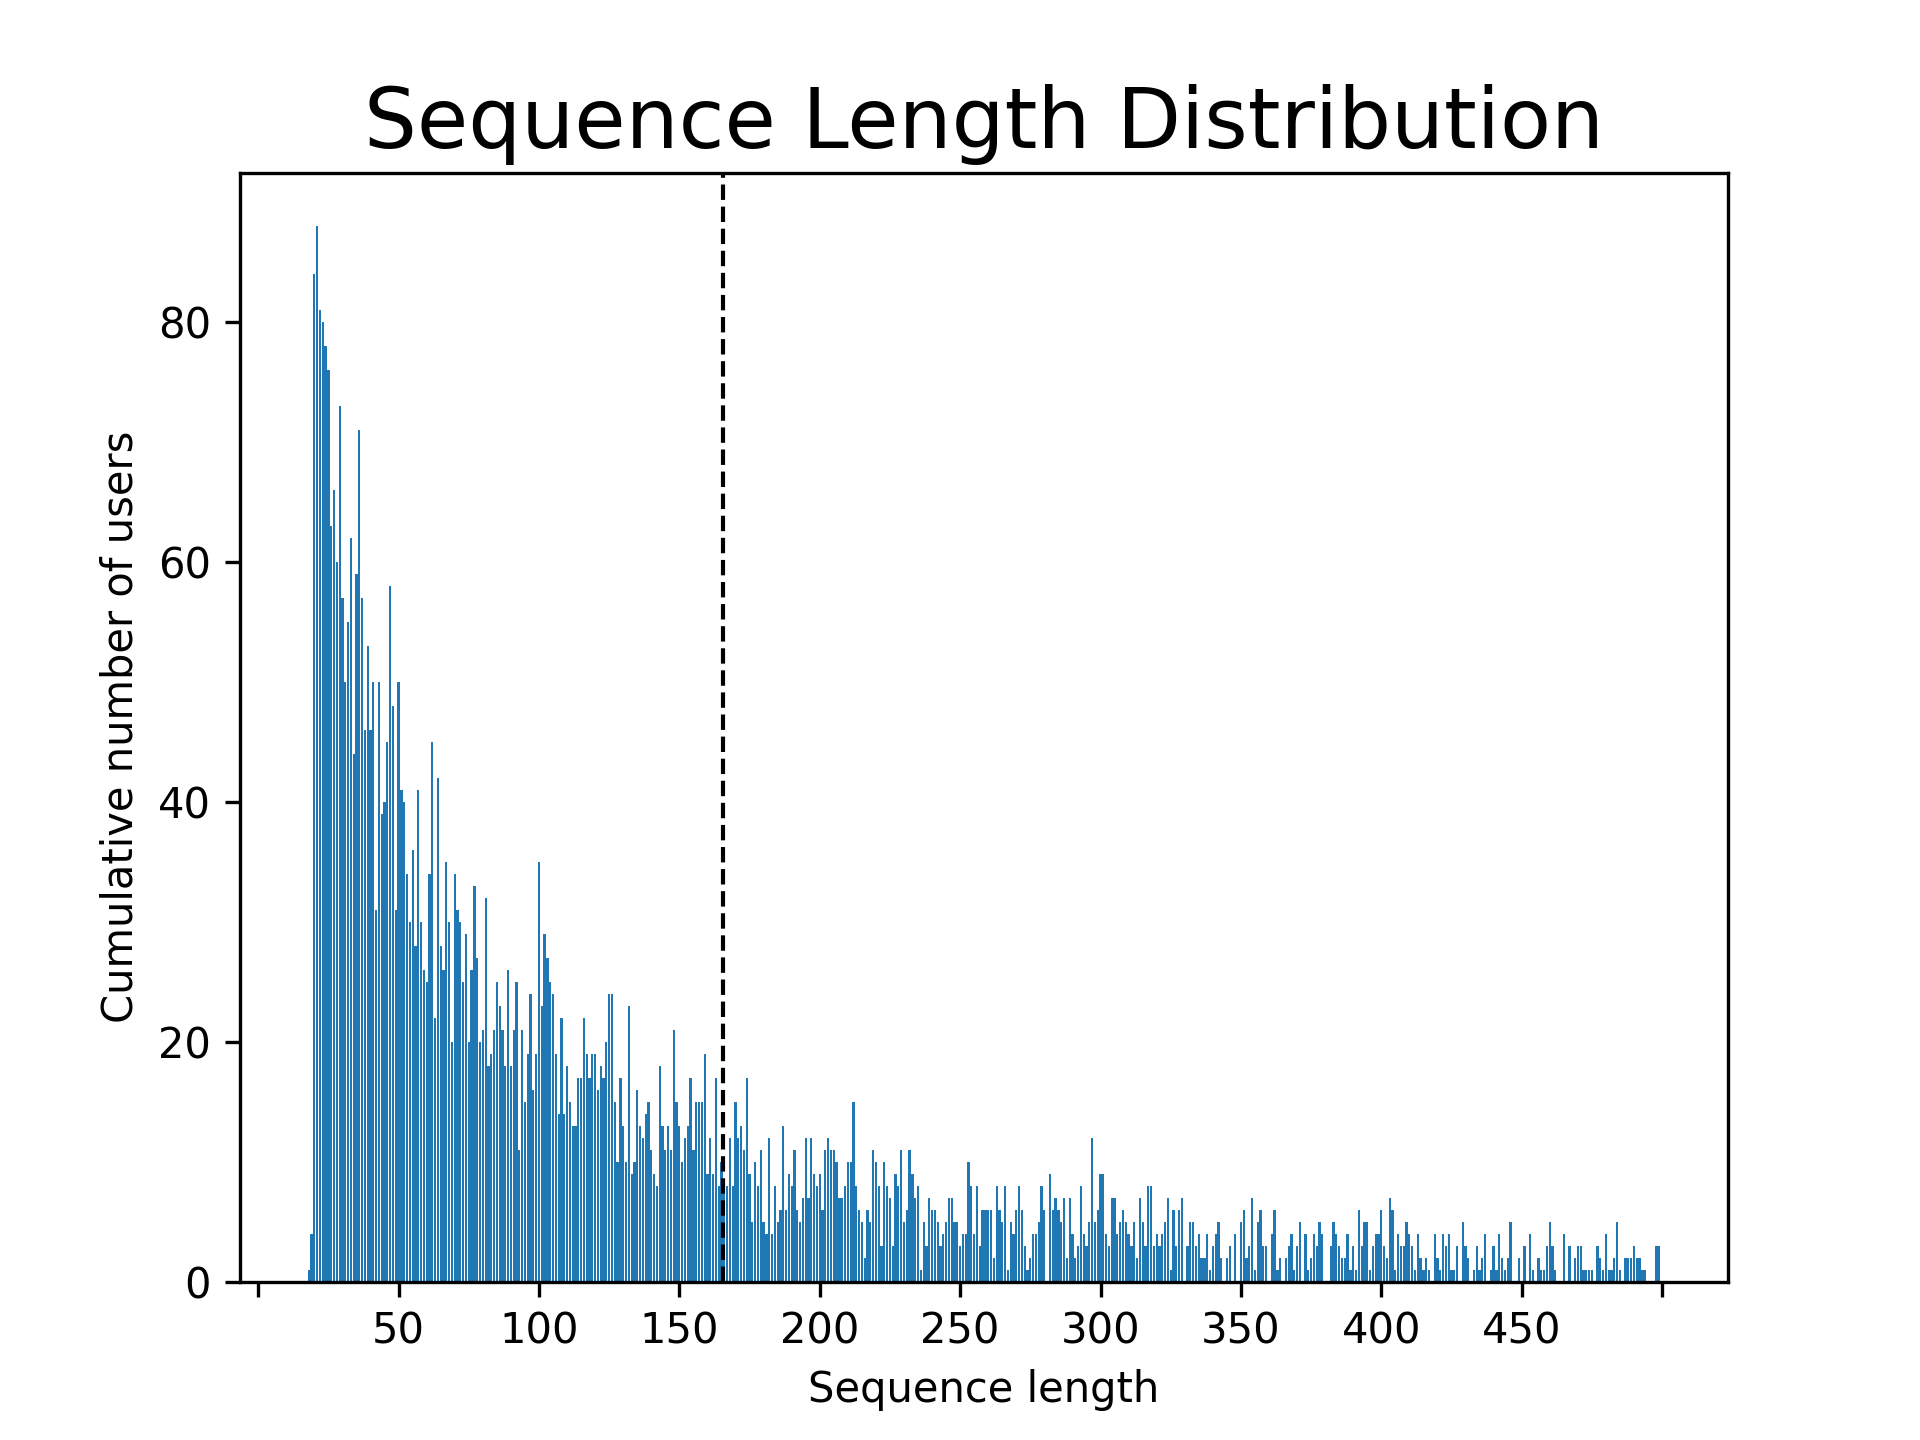
\includegraphics[width=0.5\columnwidth]{images/seq_len_dist_ml.png}}
        \subfloat[Amazon Beauty]{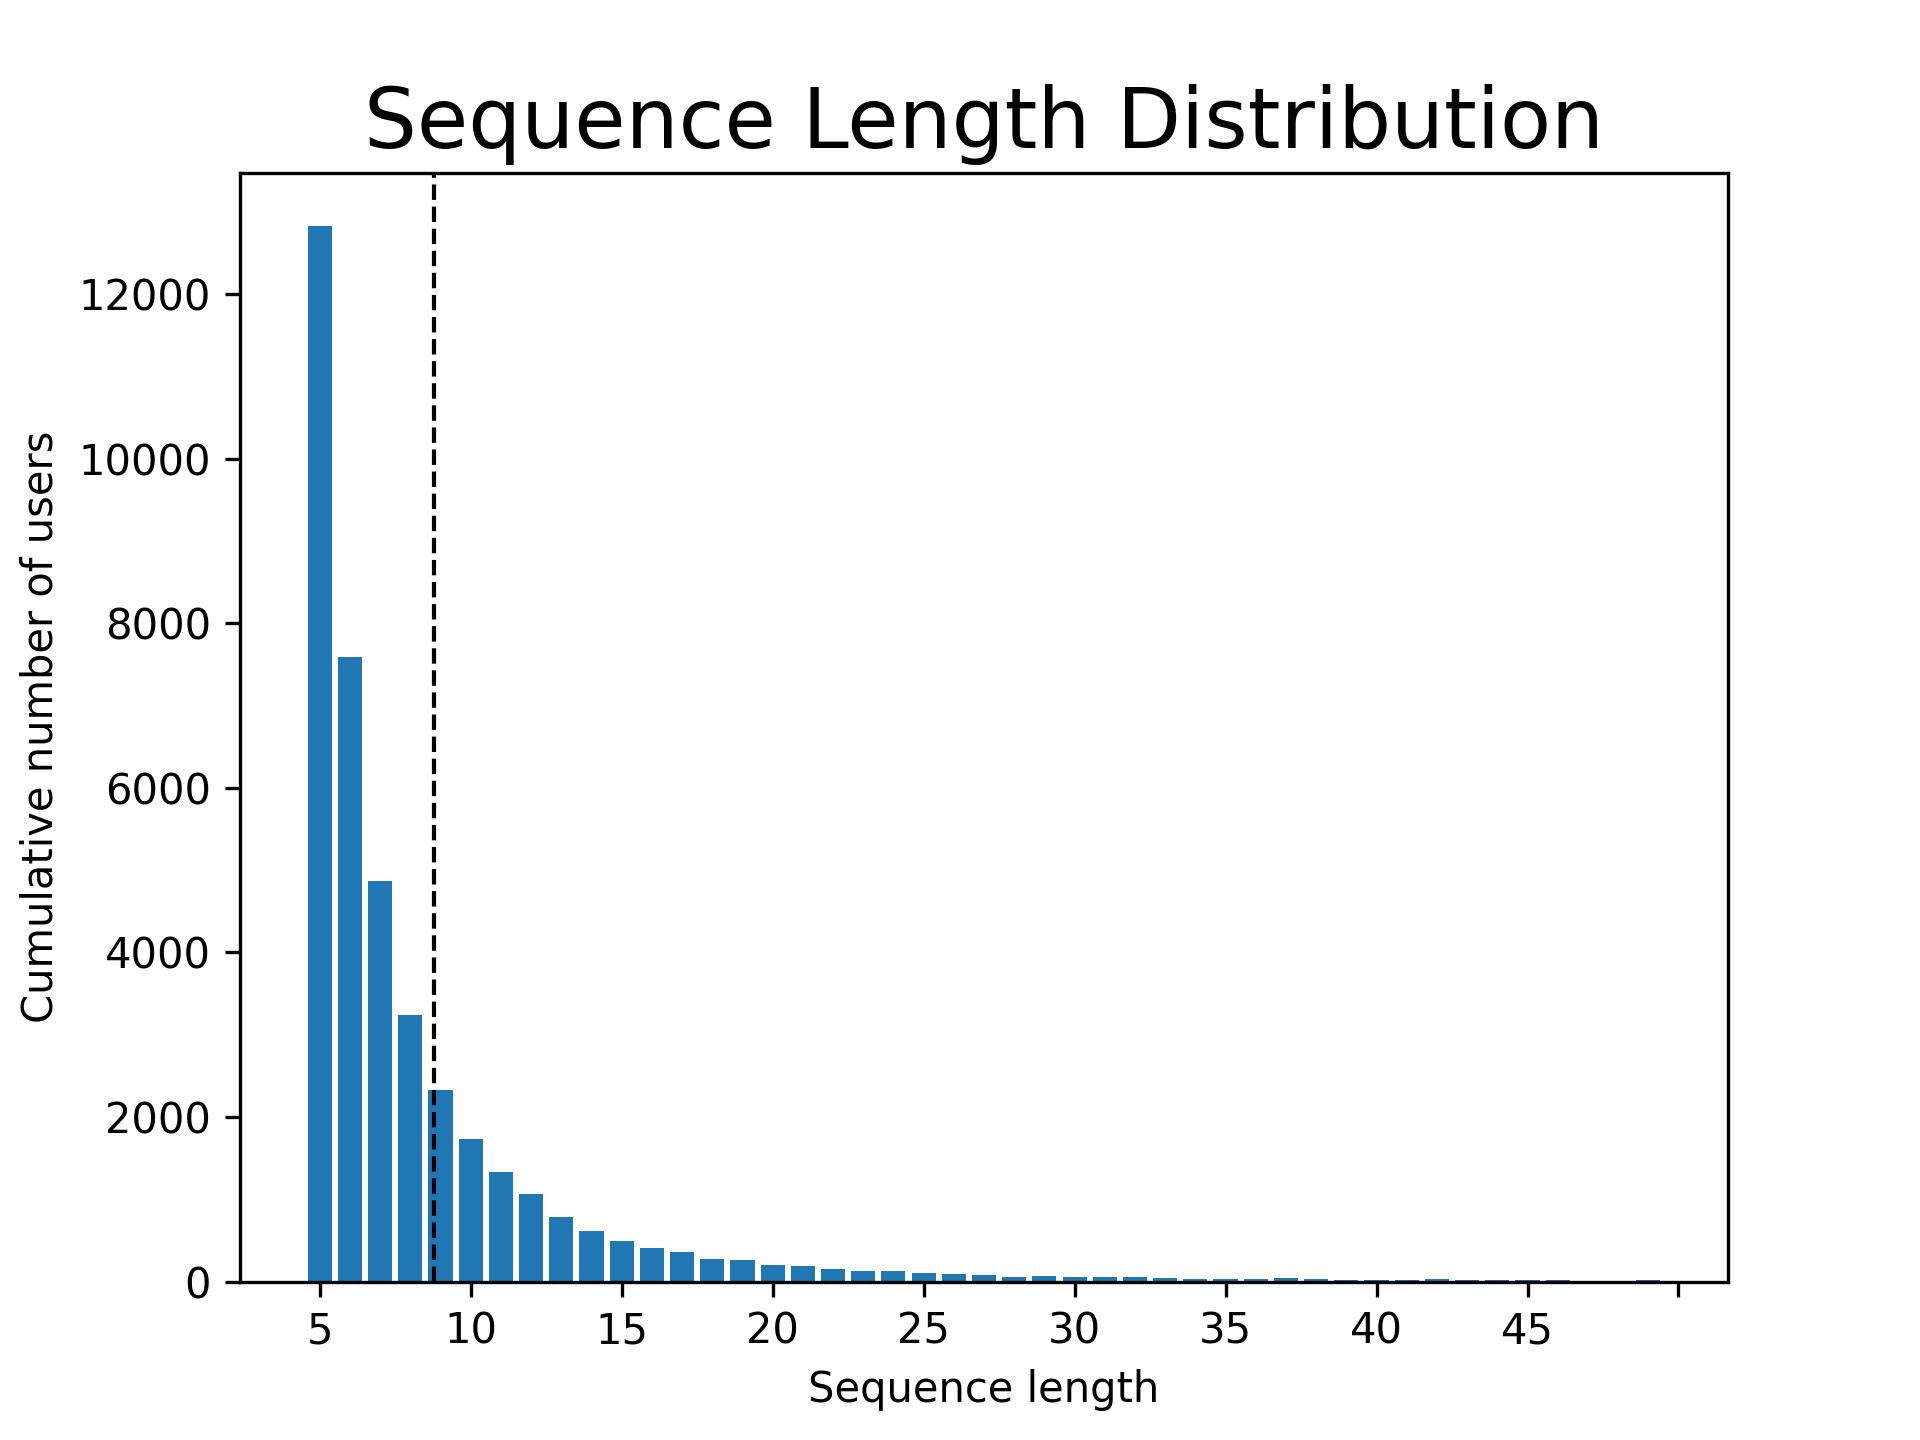
\includegraphics[width=0.5\columnwidth]{images/seq_len_dist_beauty.png}}
    \caption{The sequence length distributions of our datasets}
    \label{fig:seq_len_dist}
\end{figure}

In our case, we have only one sequence of reviews per user, namely the list of all the reviews they left, ordered by time. The sequence length is thus the number of reviews given by each user. With a mean sequence length of 8.8, the Amazon Beauty dataset consists of short sequences. In contrast, the MovieLens 1M dataset has longer sequences with a mean length of 165.5 reviews per user. We picked the two datasets to make sure our system can make accurate predictions for long and short sequences.


\subsection{Data Partition and Test Procedure}

\paragraph{Data Partition}
\label{paragraph:data_partition}
Following the literature for sequential recommender systems, we split our dataset~\cite{kang2018self, sun2019bert4rec}. The last item in the sequence of every user will be the test set, the second to last item will be the validation set, and the rest of the items we use for training.

We have created an illustrative example of the split dataset for one user, shown in Figure~\ref{fig:datasplit}.

The aim is to have our final system predict the last item in the sequence, the test set, for every user as accurately as possible.

\begin{figure}[htbp]
\centering
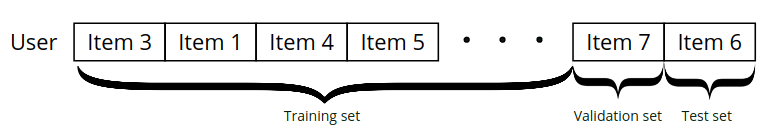
\includegraphics[width=0.8\textwidth]{images/illustrations/datasplit.png}
\caption{Example data partition for one user}
\label{fig:datasplit}
\end{figure}


\paragraph{Evaluation Procedure}
\label{paragraph:test_procedure}
Let a negative item be an item that is not in the sequence of a user meaning the user has not engaged with the item yet. We now choose 100 random negative items that the user has not engaged with and
add the last item in the sequence (the test set item) (as is common in the literature~\cite{ying2018graph}). These 101 items get fed to the system for evaluation. The system will then output a probability for every item. Ideally, the test set item gets the highest probability, which would mean that the system made the correct prediction.

We follow the same procedure for every model that we evaluate to ensure that the results are comparable. It is worth noting that the literature is not very consistent when it comes to the evaluation of models. The number of negative items used for predictions may be higher or lower. A higher number of negative items will reduce the accuracy since it becomes more difficult to make a prediction, as the number of possible items increases. Consequently, we can not let the system output a prediction for every possible item given that every dataset has a different amount of total items. Hence we limit our predictions to 100 random negative items.


\subsection{Evaluation Metrics}\label{sec:metrics}

As described in the paragraph \nameref{paragraph:test_procedure}, we feed the system 100 negative items that the user has not engaged with, plus the test set item (the last item in the user’s sequence). To demonstrate the calculation of our metrics, we have created an illustration in Figure~\ref{fig:illustration_metrics} that shows the prediction output for three random users.

\begin{figure}[htbp]
\centering
\includegraphics[width=0.9\textwidth]{images/illustration_metrics.png}
\caption{Example illustration for the computation of our metrics for three random predictions}
\label{fig:illustration_metrics}
\end{figure}

Our models use a softmax output layer which gives us a probability distribution over all the items. Each item gets a probability of being the last item in the user's sequence, and all probabilities sum up to 1. Items are then ordered by probability and ranked. The item with the highest probability gets a rank of 0. Finally, we need the rank of the actual last item, the test item, to compute our metrics.


\paragraph{Hit Rate:}
Our primary metric is the hit rate. To calculate the hit rate, we check the ratio of how many times the test set item was in the top n predictions. A higher hit rate indicates a better accuracy. Our example in Figure~\ref{fig:illustration_metrics} yields the following hit rates:

\begin{equation}
\setlength{\jot}{25pt}
    \begin{aligned}
        hit rate @1=\frac{\text{\# Hit Top 1}}{\text{\#Predictions}}=\frac{1}{3}\approx0.33 \\
        hit rate @5=\frac{\text{\# Hit Top 5}}{\text{\#Predictions}}=\frac{2}{3} \approx 0.66\\
        hit rate @10=\frac{\text{\# Hit Top 10}}{\text{\#Predictions}}=\frac{3}{3}=1.0 
    \end{aligned}
    \label{equation:hit_rate}
\end{equation}

\paragraph{Normalized Discounted Cumulative Gain (NDCG):}
To calculate the NDCG, we sum up the inverse logarithmic ranks and normalize, by dividing the result by the number of total predictions. We can determine the NDCG@n by summing up only test set items positioned in the top n predictions. A higher NDCG indicates more accurate predictions. For our example in Figure~\ref{fig:illustration_metrics}, we get the following NDCG scores:

\begin{equation}
\setlength{\jot}{25pt}
    \begin{aligned}
        NDCG@n&=\frac{ \sum\limits_{rank<n}
      \frac{1}{log_2(rank + 2)}}
      {\text{\#Predictions}} \\
        NDCG@1&=\frac{\frac{1}{log_2(0 + 2)}}{3}\approx 0.33 \\
        NDCG@5&=\frac{\frac{1}{log_2(0 + 2)}+\frac{1}{log_2(3+2)}}{3}\approx 0.48 \\
        NDCG@10&=\frac{\frac{1}{log_2(0 + 2)}+\frac{1}{log_2(3+2)}+\frac{1}{log_2(6+2)}}{3}\approx 0.59
    \end{aligned}
    \label{equation:NDCG}
\end{equation}


\paragraph{Mean Average Precision (MAP):}
The Mean Average Precision is the sum of all the inverse ranks divided by the number of predictions. Figure~\ref{fig:illustration_metrics} would give us the following score:

\begin{equation}
\setlength{\jot}{25pt}
    \begin{aligned}
        MAP=\frac{ \sum\limits_{rank}
      \frac{1}{rank + 1}}
      {\text{\#Predictions}} = \frac{\frac{1}{0+1} +\frac{1}{3+1} + \frac{1}{6+1}}{3} \approx 0.46
    \end{aligned}
    \label{equation:MAP}
\end{equation}


\paragraph{Infrastructure}
For training and evaluation, we use Google Colab Pro. The servers run Ubuntu 18.04 LTS (Bionic Beaver) and feature a Tesla P100-PCIE-16GB GPU, six Intel(R) Xeon(R) CPUs @ 2.20GHz and 27 GB of RAM. 



\section{Early Results}

\subsection{First Prototype}

So far, we have implemented a solution combining a classic mechanism---FPMC---with two state-of-the-art ML recommendation systems---BERT4Rec and Caser. BERT4Rec utilizes a bidirectional encoder representation and Caser a convolutional neural network. Our classical mechanism uses a combination of Markov chains and matrix factorization. Although the models are different, they are all able to capture sequential dependencies uniquely. With the help of matrix factorization, we have an element of personalization that can learn the preferences and similarities between different users.

Our first design choice is a hybrid-stacking approach. Stacking is a term first mentioned in the context of machine learning in 1992~\cite{wolpert1992stacked}. It has since become a popular choice for building hybrid systems~\cite{pavlyshenko2018using,sikora2015modified,dvzeroski2004combining}. The basic idea of stacking is to aggregate the outputs of different models. In the simplest form, we can take a weighted average of the output predictions~\cite{sagi2018ensemble}. To determine the weighting of the models, we use simple hand-tuning and grid search. A more sophisticated approach tries to fit the output predictions together with the help of linear regression. The outputs of the models become meta-features and the weights for the ensemble parameters of a linear function. A stacking approach using linear regression can significantly increase the accuracy of the predictions~\cite{breimanstacked,geron2019hands,sillfeature}.

\subsection{Experiment Results}

We compare our hybrid system to several state-of-the-art recommender models for the MovieLens 1M dataset. To make the evaluation fair, we follow the same evaluation procedure for every model. 

Some early tests of our hybrid system show promising results depicted in Table~\ref{tab:accuracy_hybrid}. We can see the evaluation results for the three models, that we have presented in the section~\ref{section:related_work}. For each metric, we have underlined the number of the model that scores best. We can also see the evaluation results of our hybrid system for comparison and our accuracy gain over the best model.
% 

\begin{table}[htbp!]
\centering
 \begin{tabular}{||c c c c c c c||} 
 \hline
 Model & hitrate@1 & hitrate@5 & hitrate@10 & NDCG@5 & NDCG@10 & MAP\\ [0.5ex] 
 \hline\hline
 BERT4Rec & \underline{0.3458} & \underline{0.6630} & 0.7667 & \underline{0.5156} & \underline{0.5493} & \underline{0.4905} \\ 
 %\hline
 Caser & 0.3276 & 0.6591 & \underline{0.7761} & 0.5038 & 0.5418 & 0.4780 \\
 %\hline
 FPMC & 0.2599 & 0.5812 & 0.7230 & 0.4287 & 0.4749 & 0.4103 \\
 \hline
 Hybrid & \textbf{0.3645} & \textbf{0.6855} & \textbf{0.7847} & \textbf{0.5377} & \textbf{0.5698} & \textbf{0.5197} \\ 
 %\hline 
 Accuracy Gain & 5.26\% & 3.39\% & 1.10\% & 4.28\% & 3.73\% & 5.95\% \\
 \hline
\end{tabular}
\caption{Hybrid accuracy metrics, MovieLens 1M}
\label{tab:accuracy_hybrid}
\end{table}

For better visualization we have plotted the data of the table in Figure~\ref{fig:accuracy_hybrid}.

\begin{figure}[htbp!]
\centering
\includegraphics[width=0.8\textwidth]{images/stacking_accuracy.png}
\caption{Illustration showing accuracy gain of out hybrid model compared to state of the art models for the dataset MovieLens 1M}
\label{fig:accuracy_hybrid}
\end{figure}

% description
When optimized with varying degrees of hybridization, our hybrid system can outperform the baseline scores of the state-of-the-art reference models. The accuracy gain is significant, with a 5.26\% improvement of the hitrate@1 and a 5.95\% improvement of the MAP.
% split up in analysis table vs. analysis plot

% interpretation
Hence, it appears, promisingly, that our system is able to consistently outperform the baselines while already offering a strong classic backup for guarantees.


\paragraph{Next Steps}
% 1.
Our next step will be to confirm our dominance over baselines in an online setup. We will be exploring our performance for various dynamics of the subcomponents, from small batches with close to no re-training per batch to large batches with heavy re-training.

% 2.
We will also look into letting the degree of control vary from highly automated (extensive exploration of the parameter space by the machine) to highly manual (conservative setting of the parameters by the humans). We would then use more efficient meta-learning methods for the meta optimization, e.g.,~\cite{jaderberg2017population} and related. Efficient meta learning can significantly increase the accuracy of predictions~\cite{breimanstacked,geron2019hands,sillfeature} while in the same time reducing the configuration overhead.
We also want to integrate more refined control from the classic side (internal work).

% 3.
Finally, we will be looking into the integration of the features of nodes and edges into our model (internal work).


% meta learning is there to take away painful controlling job from human, not too much for performance.
% or, rather, it's a larger space:
%   1) refined control from humans, poor exploration from machine = good perf.
%   2) coarse control from humans, deep exploration from machine = good perf.
%   3) coarse control from humans, poor exploration from machine = bad perf.
% 
% One can still get a good perf. with sheer manual tuning. It's just that it costs a lot of human time and human expertise and so it's generally a bad choice comparing to handing off the exploration to machines, aka meta learning.
% And we'll be navigating between 1) and 2), never going down to 3)–at least that's what we target.
% kind of what we said just above
%

% to merge with above. Says sensibly the same.
% Our hybridation parameters were so far set manually and we plan to move the system toward full autonomy, if desired, by optimizing more or less hybrid parameters in a space more or less broad according to the size of the parameter space defined by the user.



%%%%% Material to use later; didn't fit. Too specific for high-level sell and we don't have that yet so can't be mentioned in more concrete parts either. %%%%%

% % to move to early results. It's just one example use case for now but we should be able to support whatever other use case (marketing, medicine, knowledge base, you name it), so not particularly relevant to show off squarely on arbitrary/"random" use case of text here
% We integrate the comments from users issued when they look at a later item as the feature of the transition. The textual content can take many different forms such as the text in product reviews or social media posts. We present the design in Figure~\ref{fig:system_design_universal_Bert}. The current model encodes items without the textual content. BERT was designed originally for natural language processing tasks and can learn patterns of words in texts. We can exploit this feature to capture the full expressivity of the data, including substructures and integrating them.


